%=======================02-713 LaTeX template, following the 15-210 template==================
%
%
%
%
%    1. Update the information in section "A," put your name and the name of 
%       the class and the number of the problem set
%    2. Write your answers in section "B" below. Precede answers for all 
%       parts of a question with the command "\question{n}{desc}" where n is
%       the question number and "desc" is a short, one-line description of 
%       the problem. There is no need to restate the problem.
%    3. If a question has multiple parts, precede the answer to part x with the
%       command "\part{x}".
%

\documentclass[11pt]{article}
\usepackage[mathscr]{euscript}


\newcommand\question[2]{\vspace{.25in}\hrule\textbf{#1: #2}\vspace{.5em}\hrule\vspace{.10in}}
\renewcommand\part[1]{\vspace{.10in}\textbf{(#1)}}


% plots
\usepackage{graphicx}
\graphicspath{ {./images/} }


\usepackage{amsmath, amssymb, amsthm} %AMS packages
\usepackage{mathtools, graphicx, enumitem} %generally recommended
\usepackage{mathrsfs} %symbols I like
\usepackage{hyperref} %personal preference
\usepackage{microtype, } %recommended by stackexchange, never tried them myself
\usepackage{nag, todonotes} %workflow stuff, doesn't affect final document

% Layout
\usepackage{fancyhdr}
\usepackage[margin=1in]{geometry}
\lhead{\NAME}
\chead{\ClassNumber , Assignment \ANUM}
\rhead{Due: \duedate}
\setlength{\parindent}{0pt}
\setlength{\parskip}{5pt plus 1pt}
\setlength{\headheight}{13.6pt}
\pagestyle{fancyplain}


%-------------------------------------------<commands>--------------------------------------------------------
%%%%%%%%%%%%%%%%%%%%%%%%%%%%%%%%%%%%%%%%%											Letter Symbols
\newcommand{\R}{\mathbb{R}}
\newcommand{\N}{\mathbb{N}}
\newcommand{\Z}{\mathbb{Z}}
\newcommand{\Q}{\mathbb{Q}}
\newcommand{\C}{\mathbb{C}}
\newcommand{\F}{\mathcal{F}}
\renewcommand{\H}{\mathcal{H}} %overwrites long-umlaut diacritic
\newcommand{\eps}{\varepsilon}
\newcommand{\Exp}{\mathbb{E}}
\newcommand{\Info}{\mathcal{F}}
\renewcommand{\P}{\mathbb{P}}
%%%%%%%%%%%%%%%%%%%%%%%%%%%%%%%%%%%%%%%%%											Brackets
\newcommand{\paren}[1]{\left( #1 \right)}
\newcommand{\bracket}[1]{\left[ #1 \right]}
\newcommand{\chevron}[1]{\langle #1 \rangle}
\newcommand{\norm}[2][ ]{\left\lVert #2 \right\rVert_{#1}}
\newcommand{\abs}[1]{\left\lvert #1 \right\rvert}
\newcommand{\floor}[1]{\left\lfloor #1 \right\rfloor}
\newcommand{\ceil}[1]{\left\lceil #1 \right\rceil}
%%%%%%%%%%%%%%%%%%%%%%%%%%%%%%%%%%%%%%%%%											Operators
\DeclareMathOperator{\supp}{supp}
\DeclareMathOperator{\trace}{tr}
\DeclareMathOperator{\lspan}{span}
\DeclareMathOperator{\conv}{conv} % stands for conv, as in convex hull
\DeclareMathOperator{\Int}{int} % stands for int, as in interior of a set
\DeclareMathOperator{\cl}{cl}
\DeclareMathOperator{\sgn}{sgn}
\newcommand{\indep}{\perp \!\!\! \perp}
\newcommand{\NormCDF}[1]{\Phi \left[ #1 \right]}
%%%%%%%%%%%%%%%%%%%%%%%%%%%%%%%%%%%%%%%%%%											Aarows
\newcommand{\into}{\hookrightarrow}
\newcommand{\onto}{\twoheadrightarrow}
\newcommand{\weakly}{\rightharpoonup}
\newcommand{\isom}{\cong}
\newcommand{\restr}[1]{{\upharpoonright}_{#1}}
%\newcommand{\rest}{\big|}
%%%%%%%%%%%%%%%%%%%%%%%%%%%%%%%%%%%%%%%%%%											Common Abbreviations
\renewcommand{\th}{^\mathrm{th}} %overwrites thorn (old english letter)
\newcommand{\n}{^{-1}}
\newcommand{\half}{\frac{1}{2}}
%%%%%%%%%%%%%%%%%%%%%%%%%%%%%%%%%%%%%%%%%%											Differential Operators
\newcommand{\del}{\partial}
\newcommand{\grad}{\nabla}
\newcommand{\Laplace}{\Delta}
\renewcommand{\div}{\operatorname{div}} %overwrites division symbol
\newcommand{\dd}{\mathrm{d}}
\newcommand{\intd}{\,\dd}
\newcommand{\ddt}{\frac{\dd}{\dd t}}
\newcommand{\deriv}[2]{\frac{\dd #1}{\dd #2}} %can leave top blank, e.g. \deriv{}{x}
\newcommand{\pderiv}[2]{\frac{\partial #1}{\partial #2}} %ditto
%%%%%%%%%%%%%%%%%%%%%%%%%%%%%%%%%%%%%%%%%%											Favorite Functions and Space Names
\newcommand{\test}{\mathcal{D}}
\newcommand{\Ctest}{C_c^\infty}
\newcommand{\BMO}{\operatorname{BMO}}
\newcommand{\indic}[1]{\chi_{\{#1\}}}
\newcommand{\Leb}[2][\R^n]{L^{#2}(#1)}
%-------------------------------------------</commands>--------------------------------------------------------


\begin{document}\raggedright


%Section A==============Change the values below to match your information==================
\newcommand\NAME{Ki Hyun}  % your name
\newcommand\ClassNumber{FINM 36702}
\newcommand\ClassName{Portfolio Credit Risk: Modeling and Estimation}    
\newcommand\ANUM{2}              % the homework number
\newcommand\duedate{18:00 (CT) April 6th 2023}	% due date
%Section B==============Put your answers to the questions below here=======================

\title{Assignment \ANUM}
\author{\NAME \\ 
\ClassNumber \text{:} \ClassName}
\date{Due: \duedate}

\maketitle

%\question{1}{Description of problem}
%\part{a}

\question{1}{Std. Dev. of Defaults}

\begin{table}[h]
\centering
\begin{tabular}{|c|c|}
\hline
\multicolumn{1}{|c|}{\textbf{Correlation Matrix}} & \multicolumn{1}{c|}{\textbf{Std. Dev}} \\
\hline
Original & \textbf{1.2} \\
\hline
Identity Matrix$^*$ & \textbf{0.98} \\
\hline
\end{tabular}
\caption{Correlation and Std. Dev. of Defaults}
\end{table}

* The identity matrix mentioned above would be in the form:

\[
\begin{bmatrix}
1 & 0 & 0 & 0 & 0 \\
0 & 1 & 0 & 0 & 0 \\
0 & 0 & 1 & 0 & 0 \\
0 & 0 & 0 & 1 & 0 \\
0 & 0 & 0 & 0 & 1 \\
\end{bmatrix}
\]

\question{2}{$\rho$ vs Risk}

\begin{figure}[h]
\centering
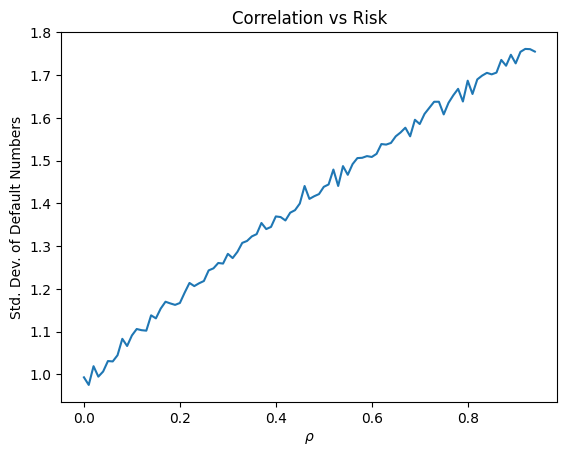
\includegraphics[scale=0.51]{Q2.png}
\caption{Std. Dev. of Defaults as a function of $\rho$}
\label{Fig:Q2}
\end{figure}

\newpage

\question{3}{Exposures in Loan}

\part{i: $\P[D_4 = 1, D_5 = 1]$}

$\P[D_4 = 1, D_5 = 1]$ can be calculated analytically 
using the multivariate normal distribution of the latent variables
of all the 5 firms.

If the latent variable for firm $i$ is $d_i$, the distribution can
be represented as:

$$
\mathbf{d} = \begin{pmatrix}
d_1 \\
d_2 \\
d_3 \\
d_4 \\
d_5
\end{pmatrix}
\sim
MVN(\mathbf{\mu}, \mathbf{\Sigma})
$$

Here,

$$
\mathbf{\mu} = \begin{pmatrix}
0 \\
0 \\
0 \\
0 \\
0
\end{pmatrix}, \
\mathbf{\Sigma} = \begin{bmatrix}
1 & 0.15 & 0.2 & 0.25 & 0.3 \\
0.15 & 1 & 0.25 & 0.3 & 0.35 \\
0.2 & 0.25 & 1 & 0.35 & 0.4 \\
0.25 & 0.3 & 0.35 & 1 & 0.45 \\
0.3 & 0.35 & 0.4 & 0.45 & 1 \\
\end{bmatrix}
$$

Now the mathematical form for $\P[D_4 = 1, D_5 = 1]$
can be expressed as:

$$
\begin{aligned}
& \P[D_4 = 1, D_5 = 1] \\
=& \int_{-\infty}^{\Phi^{-1}(PD_5)}
\int_{-\infty}^{\Phi^{-1}(PD_4)}
\int_{-\infty}^{\infty}
\int_{-\infty}^{\infty}
\int_{-\infty}^{\infty}
\frac{1}{(2\pi)^{5/2}|\mathbf{\Sigma}|^{1/2}}\exp\left(-\frac{1}{2}(\mathbf{d}-\mathbf{\mu})^{\mathrm{T}}\mathbf{\Sigma}^{-1}(\mathbf{d}-\mathbf{\mu})\right) \\
& d d_1 d d_2 d d_3 d d_4 d d_5 \\
=& \int_{-\infty}^{\Phi^{-1}(0.5)}
\int_{-\infty}^{\Phi^{-1}(0.4)}
\int_{-\infty}^{\infty}
\int_{-\infty}^{\infty}
\int_{-\infty}^{\infty}
\frac{1}{(2\pi)^{5/2}|\mathbf{\Sigma}|^{1/2}}\exp\left(-\frac{1}{2}(\mathbf{d}-\mathbf{\mu})^{\mathrm{T}}\mathbf{\Sigma}^{-1}(\mathbf{d}-\mathbf{\mu})\right) \\
& d d_1 d d_2 d d_3 d d_4 d d_5 \\
&(\because PD_4 = 0.4, PD_5 = 0.5) \\
\approx & 0.27
\end{aligned}
$$

$$
\therefore
\P[D_4 = 1, D_5 = 1]
\approx 0.27
$$

\part{ii: $\P[D_4 = 1, D_5 = 1 \mid D_3 = 1]$}

Using the definition of conditional probability:

$$
\P[D_4 = 1, D_5 = 1 \mid D_3 = 1] =
\frac{\P[D_4 = 1, D_5 = 1, D_3 = 1]}{\P[D_3 = 1]}
$$

\newpage

Here,

$$
\begin{aligned}
& \P[D_4 = 1, D_5 = 1, D_3 = 1] \\
=& \int_{-\infty}^{\Phi^{-1}(PD_5)}
\int_{-\infty}^{\Phi^{-1}(PD_4)}
\int_{-\infty}^{\Phi^{-1}(PD_3)}
\int_{-\infty}^{\infty}
\int_{-\infty}^{\infty}
\frac{1}{(2\pi)^{5/2}|\mathbf{\Sigma}|^{1/2}}\exp\left(-\frac{1}{2}(\mathbf{d}-\mathbf{\mu})^{\mathrm{T}}\mathbf{\Sigma}^{-1}(\mathbf{d}-\mathbf{\mu})\right) \\
& d d_1 d d_2 d d_3 d d_4 d d_5 \\
=& \int_{-\infty}^{\Phi^{-1}(0.5)}
\int_{-\infty}^{\Phi^{-1}(0.4)}
\int_{-\infty}^{\Phi^{-1}(0.3)}
\int_{-\infty}^{\infty}
\int_{-\infty}^{\infty}
\frac{1}{(2\pi)^{5/2}|\mathbf{\Sigma}|^{1/2}}\exp\left(-\frac{1}{2}(\mathbf{d}-\mathbf{\mu})^{\mathrm{T}}\mathbf{\Sigma}^{-1}(\mathbf{d}-\mathbf{\mu})\right) \\
& d d_1 d d_2 d d_3 d d_4 d d_5 \\
&(\because PD_4 = 0.4, PD_5 = 0.5, PD_3 = 0.3)
\end{aligned}
$$

Moreover,

$$
\begin{aligned}
& \P[D_3 = 1] \\
=& \int_{-\infty}^{\Phi^{-1}(PD_3)}
\int_{-\infty}^{\infty}
\int_{-\infty}^{\infty}
\int_{-\infty}^{\infty}
\int_{-\infty}^{\infty}
\frac{1}{(2\pi)^{5/2}|\mathbf{\Sigma}|^{1/2}}\exp\left(-\frac{1}{2}(\mathbf{d}-\mathbf{\mu})^{\mathrm{T}}\mathbf{\Sigma}^{-1}(\mathbf{d}-\mathbf{\mu})\right)
d d_1 d d_2 d d_4 d d_5 d d_3 \\
=& \int_{-\infty}^{\Phi^{-1}(0.3)}
\int_{-\infty}^{\infty}
\int_{-\infty}^{\infty}
\int_{-\infty}^{\infty}
\int_{-\infty}^{\infty}
\frac{1}{(2\pi)^{5/2}|\mathbf{\Sigma}|^{1/2}}\exp\left(-\frac{1}{2}(\mathbf{d}-\mathbf{\mu})^{\mathrm{T}}\mathbf{\Sigma}^{-1}(\mathbf{d}-\mathbf{\mu})\right)
d d_1 d d_2 d d_4 d d_5 d d_3 \\
&(\because PD_3 = 0.3)
\end{aligned}
$$

Therefore,

$$
\begin{aligned}
&\P[D_4 = 1, D_5 = 1 \mid D_3 = 1] \\
=& \frac{\P[D_4 = 1, D_5 = 1, D_3 = 1]}{\P[D_3 = 1]} \\
=& \frac{
\int_{-\infty}^{\Phi^{-1}(0.5)}
\int_{-\infty}^{\Phi^{-1}(0.4)}
\int_{-\infty}^{\Phi^{-1}(0.3)}
\int_{-\infty}^{\infty}
\int_{-\infty}^{\infty}
\frac{1}{(2\pi)^{5/2}|\mathbf{\Sigma}|^{1/2}}\exp\left(-\frac{1}{2}(\mathbf{d}-\mathbf{\mu})^{\mathrm{T}}\mathbf{\Sigma}^{-1}(\mathbf{d}-\mathbf{\mu})\right)
d d_1 d d_2 d d_3 d d_4 d d_5
}
{
\int_{-\infty}^{\Phi^{-1}(0.3)}
\int_{-\infty}^{\infty}
\int_{-\infty}^{\infty}
\int_{-\infty}^{\infty}
\int_{-\infty}^{\infty}
\frac{1}{(2\pi)^{5/2}|\mathbf{\Sigma}|^{1/2}}\exp\left(-\frac{1}{2}(\mathbf{d}-\mathbf{\mu})^{\mathrm{T}}\mathbf{\Sigma}^{-1}(\mathbf{d}-\mathbf{\mu})\right)
d d_1 d d_2 d d_4 d d_5 d d_3
} \\
\approx & 0.44
\end{aligned}
$$

$$
\therefore
\P[D_4 = 1, D_5 = 1 \mid D_3 = 1]
\approx 0.44
$$

\part{iii: Portfolio Expected Loss Rate}

Given the ELGD and Exposure of the portfolio across the 7 loans,
the expected loss at default for each firm could be summarized to:

\begin{center}
\begin{tabular}{|c|c|}
\hline
Firm & Expected Loss at Default \\
\hline
Firm 1 & 70 \\
Firm 2 & 120 \\
Firm 3 & 150 \\
Firm 4 & 280 \\
Firm 5 & 220 \\
\hline
\end{tabular}
\end{center}

Now using 1,000,000 simulations from the $MVN(\mathbf{\mu}, 
\mathbf{\Sigma})$ and comparing each result with the Probabilities
of Default ($PD_1, \dots, PD_5$) to get 1,000,000 vectors in the form:

$$
\mathbf{D}_{sim = j} =
\begin{pmatrix}
D_{1, sim = j} \\
D_{2, sim = j} \\
D_{3, sim = j} \\
D_{4, sim = j} \\
D_{5, sim = j}
\end{pmatrix}
$$

Here, $D_{i, sim = j}$ will represent if firm $i$ has defaulted
in the $j^{th}$ simulation:

$$
D_{i, sim = j} = \begin{cases}
1 & \text{Firm } i \text{ Defaulted in the jth simulation} \\
0 & \text{Otherwise in the jth simulation} \\
\end{cases}
$$

Now, if we let $\Exp[\text{Loss}]$ be the vector:

$$
\Exp[\text{Loss}] = 
\begin{pmatrix}
70 \\
120 \\
150 \\
280 \\
220
\end{pmatrix}
$$

Our expected \textbf{portfolio} loss from the simulation will be:

$$
\sum_{j = 1}^{1,000,000}
\mathbf{D}_{sim = j} \cdot \Exp[\text{Loss}]
$$

Moreover, the expected loss rate can be estimated as:

$$
\Exp[\text{Loss Rate}] =
\frac{2800}
{\sum_{j = 1}^{1,000,000}\mathbf{D}_{sim = j} \cdot \Exp[\text{Loss}]}
\approx 0.11
$$

\part{iv: Dcorr}

First, similar to (part i), we can get $PDJ_{3, 4}$ as:

$$
\begin{aligned}
& \P[D_3 = 1, D_4 = 1] \\
=& \int_{-\infty}^{\Phi^{-1}(PD_4)}
\int_{-\infty}^{\Phi^{-1}(PD_3)}
\int_{-\infty}^{\infty}
\int_{-\infty}^{\infty}
\int_{-\infty}^{\infty}
\frac{1}{(2\pi)^{5/2}|\mathbf{\Sigma}|^{1/2}}\exp\left(-\frac{1}{2}(\mathbf{d}-\mathbf{\mu})^{\mathrm{T}}\mathbf{\Sigma}^{-1}(\mathbf{d}-\mathbf{\mu})\right) \\
& d d_1 d d_2 d d_5 d d_3 d d_4 \\
=& \int_{-\infty}^{\Phi^{-1}(0.4)}
\int_{-\infty}^{\Phi^{-1}(0.3)}
\int_{-\infty}^{\infty}
\int_{-\infty}^{\infty}
\int_{-\infty}^{\infty}
\frac{1}{(2\pi)^{5/2}|\mathbf{\Sigma}|^{1/2}}\exp\left(-\frac{1}{2}(\mathbf{d}-\mathbf{\mu})^{\mathrm{T}}\mathbf{\Sigma}^{-1}(\mathbf{d}-\mathbf{\mu})\right) \\
& d d_1 d d_2 d d_5 d d_3 d d_4 \\
&(\because PD_3 = 0.3, PD_4 = 0.4)
\end{aligned}
$$

Now using the properties of a Bernoulli distribution:

$$
\begin{aligned}
&Dcorr_{3, 4} \\
=& \frac{PDJ_{3, 4} - PD_3 \cdot PD_4}
{\sqrt{PD_3 (1 - PD_3)}\sqrt{PD_4 (1 - PD_4)}} \\
=& \frac{\int_{-\infty}^{\Phi^{-1}(0.4)}
\int_{-\infty}^{\Phi^{-1}(0.3)}
\int_{-\infty}^{\infty}
\int_{-\infty}^{\infty}
\int_{-\infty}^{\infty}
\frac{1}{(2\pi)^{5/2}|\mathbf{\Sigma}|^{1/2}}\exp\left(-\frac{1}{2}(\mathbf{d}-\mathbf{\mu})^{\mathrm{T}}\mathbf{\Sigma}^{-1}(\mathbf{d}-\mathbf{\mu})\right)
d d_1 d d_2 d d_5 d d_3 d d_4}
{\sqrt{0.3 (1 - 0.3) \cdot 0.4 (1 - 0.4)}} \\
& - \frac{0.3 \cdot 0.4}{\sqrt{0.3 (1 - 0.3) \cdot 0.4 (1 - 0.4)}} \\
\approx & 0.22
\end{aligned}
$$

$$
\therefore
Dcorr_{3, 4}
\approx 0.22
$$

\question{4}{36702 Distribution}

The joint probability density of $x$ and $y$ was given as:

\begin{equation} \tag{4 - 0}
f_{x, y}[x, y] = \frac{1 + 3x - y}{2}
\end{equation}

From this, we can derive the marginal density as:

$$
f_x[x] = \int_0^1 \frac{1 + 3x - y}{2} dy
= \frac{3}{2} x + \frac{1}{4}
$$

and

$$
f_y[y] = \int_0^1 \frac{1 + 3x - y}{2} dx
= -\frac{1}{2} y + \frac{5}{4}
$$

The marginal density now gives way to marginal CDF:

$$
F_x[z] = \int_0^z \frac{3}{2} x + \frac{1}{4} dx
= \frac{3}{4} z^2 + \frac{1}{4} z
$$

and

$$
F_y[z] = \int_0^z -\frac{1}{2} y + \frac{5}{4} dy
= -\frac{1}{4} z^2 + \frac{5}{4} z
$$

Now from the marginal CDF, we get get the inverse CDF 
(quantile function) as:

$$
F^{-1}_x[p]:
p = \frac{3}{4} z^2 + \frac{1}{4} z, \
0 \leq p, z \leq 1
$$

\begin{equation} \tag{4 - 1}
\Leftrightarrow
F^{-1}_x[p] =
\frac{-1 + \sqrt{1 + 48p}}{6}
\end{equation}

\newpage

Moreover,

$$
F^{-1}_y[p]:
p = -\frac{1}{4} z^2 + \frac{5}{4} z, \
0 \leq p, z \leq 1
$$

\begin{equation} \tag{4 - 2}
\Leftrightarrow
F^{-1}_y[p] =
\frac{5 - \sqrt{25 - 16p}}{2}
\end{equation}

\part{i: PDJ}

The probability of default for $x$ and $y$ were given as
$PD_x = 0.1$ and $PD_y = 0.2$.

Using this knowledge and the above, we can express the PDJ as:

$$
\begin{aligned}
&PDJ_{x, y} \\
&= \int_0^{F^{-1}_y[0.2]}
\int_0^{F^{-1}_x[0.1]}
f_{x, y}[x, y] dx dy \\
&= \int_0^{F^{-1}_y[0.2]}
\int_0^{F^{-1}_x[0.1]}
\frac{1 + 3x - y}{2} dx dy \\
&(\because (4 - 0)) \\
&= \int_0^{\frac{5 - \sqrt{25 - 16 \cdot 0.2}}{2}}
\int_0^{\frac{-1 + \sqrt{1 + 48 \cdot 0.1}}{6}}
\frac{1 + 3x - y}{2} dx dy \\
&(\because (4 - 1), \ (4 - 2)) \\
& \approx 0.025
\end{aligned}
$$

\part{ii: Dcorr}

Using the PDJ above, the Dcorr can be calculated using the 
characteristics of a Bernoulli distribution as:

$$
\begin{aligned}
&Dcorr_{x, y} \\
=& \frac{PDJ_{x, y} - PD_x \cdot PD_y}
{\sqrt{PD_x (1 - PD_x)}\sqrt{PD_y (1 - PD_y)}} \\
\approx & 0.039
\end{aligned}
$$

\newpage

\part{iii: $\rho$}

In order to find the $\rho$ we need to declare another
set of latent variables that are Gaussian copula.

If we let those latent variables be $n_x$ and $n_y$:

$$
\mathbf{n} = \begin{pmatrix}
n_x \\
n_y \\
\end{pmatrix}
\sim
MVN(\mathbf{\mu}, \mathbf{\Sigma})
$$

where

$$
\mathbf{\mu} = \begin{pmatrix}
0 \\
0 \\
\end{pmatrix}, \
\mathbf{\Sigma} = \begin{bmatrix}
1 & \rho \\
\rho & 1 \\
\end{bmatrix}
$$

$PDJ_{x, y}$ can be expressed using the above 
Gaussian distribution as:

$$
PDJ_{x, y} = \int_{-\infty}^{\Phi^{-1}[PD_y]}
\int_{-\infty}^{\Phi^{-1}[PD_x]}
\frac{1}{(2\pi)|\mathbf{\Sigma}|^{1/2}}
\exp\left(-\frac{1}{2}(\mathbf{n}-\mathbf{\mu})^{\mathrm{T}}
\mathbf{\Sigma}^{-1}(\mathbf{n}-\mathbf{\mu})\right) dx dy
$$

Now using the calculated $PDJ_{x, y}$ value and the given
$PD_x$ and $PD_y$ values, the equation above becomes:

$$
0.025 = \int_{-\infty}^{\Phi^{-1}[0.2]}
\int_{-\infty}^{\Phi^{-1}[0.1]}
\frac{1}{(2\pi)|\mathbf{\Sigma}|^{1/2}}
\exp\left(-\frac{1}{2}(\mathbf{n}-\mathbf{\mu})^{\mathrm{T}}
\mathbf{\Sigma}^{-1}(\mathbf{n}-\mathbf{\mu})\right) dx dy
$$

Using python, the $\rho$ that satisfies the above equation
turns out to be approximately $0.090$.

$$
\therefore
\rho \approx 0.090
$$

\end{document}

$$
\begin{aligned}
\end{aligned}
$$